\subsection{linearised Model}
The Non-linear model presented in \cref{sec:Non-linear} is linearised to fit the standard state space model:
\begin{equation*}
	\dot{x}=Ax+Bu
\end{equation*}
Linearisation of our system is done via a $ 1^{st} $-order Taylor approximation: 
\begin{equation}\label{eq:TaylorSeries}
	\dot{x} \approx f(x_0) + \nabla f\bigg\rvert_{x_0} (x-x_0)
\end{equation}
Linearising \cref{eq:NonLinearModelWithTank} results in the following approximation:
\begin{equation}\label{eq:LinearisedModelWithTank}
	\begin{split}
	\dot{q}_n \approx &-\mathcal{P}\Phi\Bigg(a_1\omega_0 + \Big(|q_0|+\text{sign}(q_0)q_0\Big)\\
	&\Bigg(K_\lambda + a_2 + \frac{1}{(K_v OD_0)^2}\Bigg) \tilde{q}_n \Bigg)\\
	&- \mathcal{P}\Phi\Bigg(\Big(a_1 q_0 + 2a_0\omega_0\Big) \tilde{\omega}\Bigg)
	\end{split}
\end{equation}

\begin{figure}[h]
	\centering
	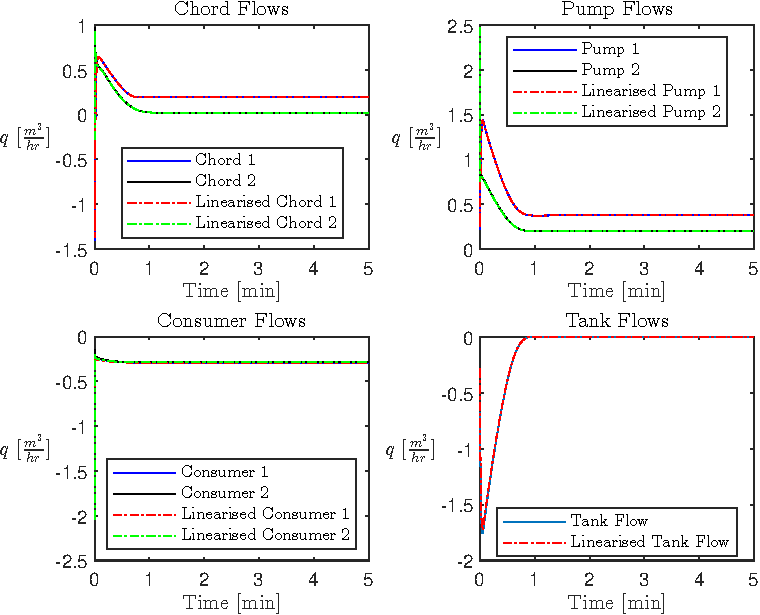
\includegraphics[width=\linewidth]{Graphics/NominalFlows.pdf}
	\caption{Comparison of non-linear and linearised model behaviour}
	\label{fig:CompNonlinLin}
\end{figure}